\documentclass[UTF8]{ctexart}
\usepackage{amsmath}
\usepackage{diagbox}
\usepackage{textcomp}
\usepackage{graphicx}
\usepackage{float}
\usepackage{caption}
\usepackage{adjustbox}
\usepackage{subfigure}
\usepackage{geometry}
\usepackage{pifont}
\usepackage{chngpage}
\usepackage{bm}
\begin{document}
\renewcommand{\thefootnote}{\fnsymbol{footnote}}
\newgeometry{left=2.5cm,bottom=4cm,right=2.5cm}
%\pagestyle{plain}
\linespread{1.4}
\title{\vspace{-5em}\heiti套件的使用实验报告\vspace{-2.5em}}
\date{}
\maketitle
\begin{center}
{\fangsong 徐浩博\quad 软件02\quad2020010108}
\end{center}

\subsubsection*{摘要}
{\kaishu\normalsize  本实验旨在通过于FPGA板上模拟质数电路,使我们掌握FPGA、Quantus II等实验套件及实验用软件的使用方法,并且进一步巩固电路图的画法、真值表、卡诺图的概念及应用等知识,并使得我们第一次亲手独立设计出实用电路,了解电路设计的基本流程和验证方法.}
\subsubsection*{关键词:Quartus II\quad 卡诺图\quad质数电路\quad 功能仿真 \quad FPGA\quad \vspace{1.5em}}


\section{实验仪器}
安装Quartus II的计算机\par
FPGA板\par
适配FPGA板的电源线、数据线
\par

\section{实验内容}

\subsection*{ A) 电路原理图}
题目要求设计质数判断电路,用$x=(ABCD)_2$表示要求判断的数,并且令x为质数时F取值为1,反之为0,如此则可写出质数判断电路的真值表:
\begin{center}\begin{table}[H]
    
\hspace{6em}
	\begin{minipage}[t]{0.4\textwidth}
    \begin{tabular}{c|c c c c|c}
        \hline
        数字 & A & B & C & D & F\\
        \hline
        0&0&0&0&0&0\\
        1&0&0&0&1&0\\
        2&0&0&1&0&1\\
        3&0&0&1&1&1\\
        4&0&1&0&0&0\\
        5&0&1&0&1&1\\
        6&0&1&1&0&0\\
        7&0&1&1&1&1\\
        \hline
    \end{tabular}
    \end{minipage}
    \hfill
	\begin{minipage}[t]{0.4\textwidth}
    \begin{tabular}{c|c c c c|c}
        \hline
        数字 & A & B & C & D & F\\
        \hline
        8&1&0&0&0&0\\
        9&1&0&0&1&0\\
        10&1&0&1&0&0\\
        11&1&0&1&1&1\\
        12&1&1&0&0&0\\
        13&1&1&0&1&1\\
        14&1&1&1&0&0\\
        15&1&1&1&1&0\\
        \hline
    \end{tabular}
    \end{minipage}
\end{table}\end{center}
\vspace{-2em}
由此可以得出$F=A'B'CD'+A'B'CD+A'BC'D+A'BCD+A'BCD+AB'CD+ABC'D$. 画出卡诺图如下:
\begin{table}[H]\begin{center}
\begin{tabular}{|c|c c c c|}
    \hline
    \diagbox[width = 5em,height=2em]{AB}{CD}&00&01&11&10\\
    \hline
    00&0&0&1&1\\
    01&0&1&1&0\\
    11&0&1&0&0\\
    10&0&0&1&0\\
    \hline
\end{tabular}
\end{center}\end{table}
第2列2、3行合并得到BC'D,第3列1、2行合并得到A'CD,第3列1、4行合并得到B'CD,第1行3、4列合并得到A'B'C,综合以上:
\[F=A'B'C+A'CD+BC'D+B'CD\]
由此,可以用或门将A'B'C、A'CD、BC'D、B'CD连接,得到如下电路图:
\begin{figure}[H]\centering
    {
    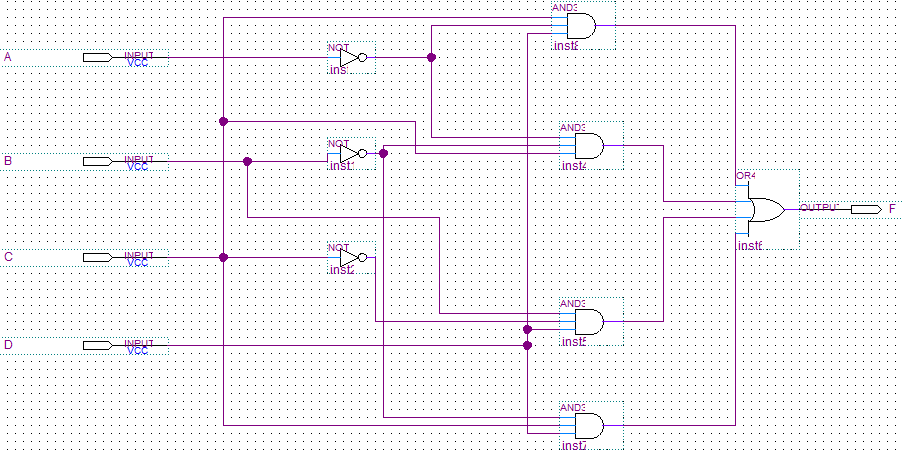
\includegraphics[scale=1.0]{curcuit.PNG}
    }
    \end{figure}

\subsection*{ B) 功能仿真输入/输出波形}

\begin{figure}[H]\centering
    {
    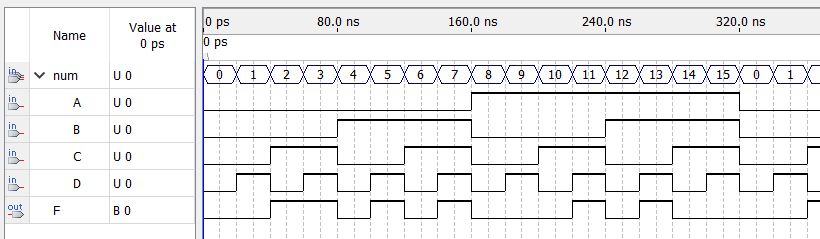
\includegraphics[scale=0.9]{wave.PNG}
    }
\end{figure}
由图,可以明显看出,2、3、5、7、11、13对应的F显示为高电平,为质数;其他各个数显示为低电平,不为质数。

\subsection*{ C) 下载到FPGA上的实现效果}
我们用$(ABCD)_2$表示数字,$A$为最高位,$D$为最低位,并将其分别对应到$SW1-SW4$四个按钮上;同时我们将显示结果$F$对应到$LED3$上,$LED$灯亮表示该数为质数,反之不是。如下图标注所示:
\begin{figure}[H]
    \centering{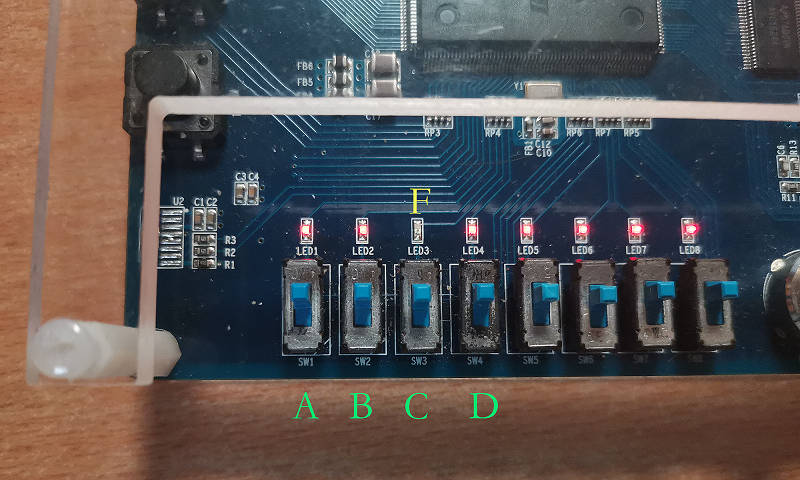
\includegraphics[scale=0.4]{0.png}}
\end{figure}
FPGA显示0-15是否为质数的效果如下所示:
\begin{figure}[H]\centering
    {
    %https://blog.csdn.net/a386115360/article/details/89358723
    \newgeometry{a4paper,left=3cm,right=0cm}
    \vspace{-1em}
    \subfigcapskip=-10pt
    \subfigure[0]{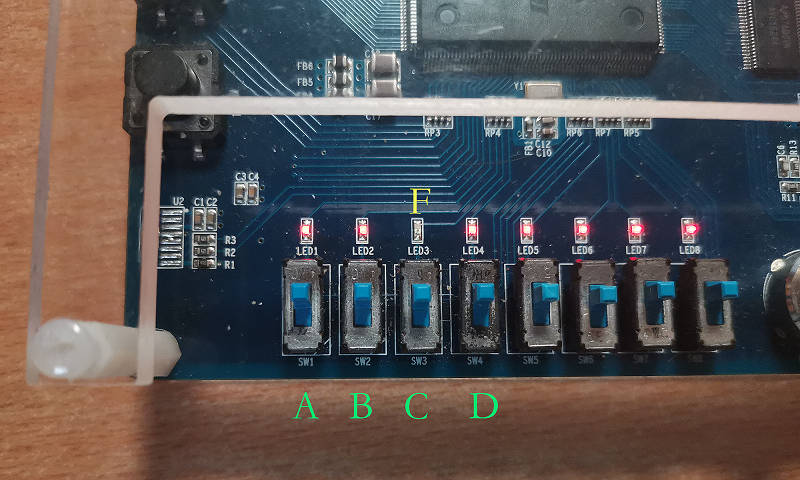
\includegraphics[scale=0.36]{0.png}}\hspace{0.3mm}
    \subfigure[1]{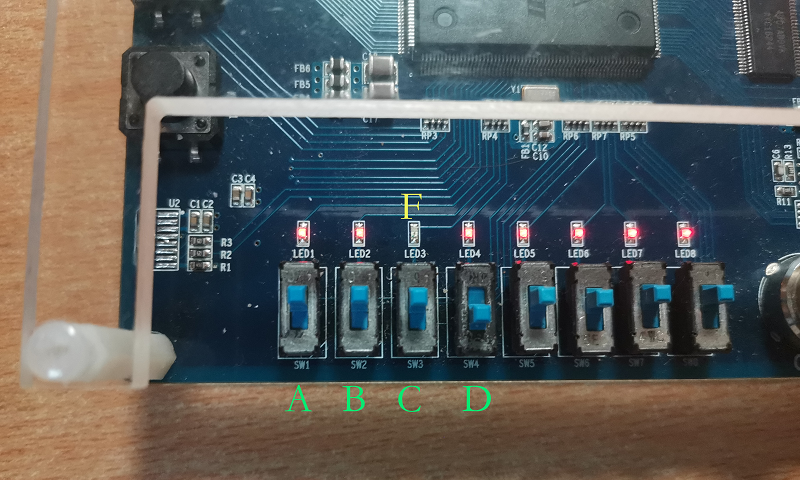
\includegraphics[scale=0.36]{1.png}}\hspace{0.3mm}
    \subfigure[2]{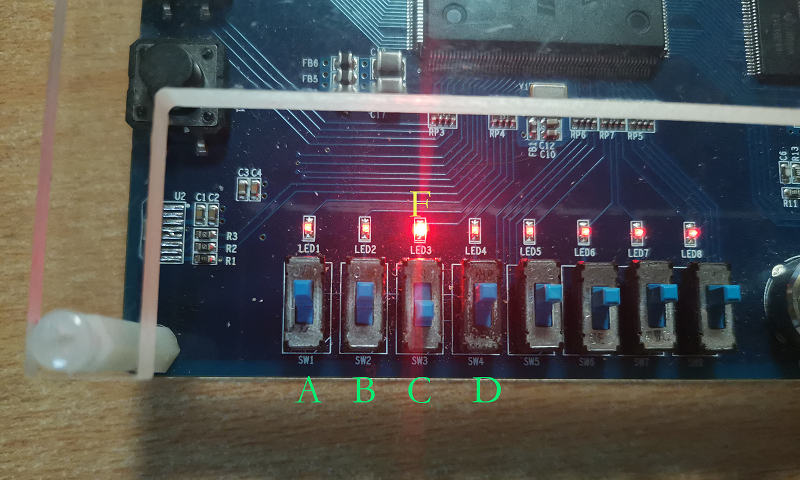
\includegraphics[scale=0.36]{2.png}}\hspace{0.3mm}
    \subfigure[3]{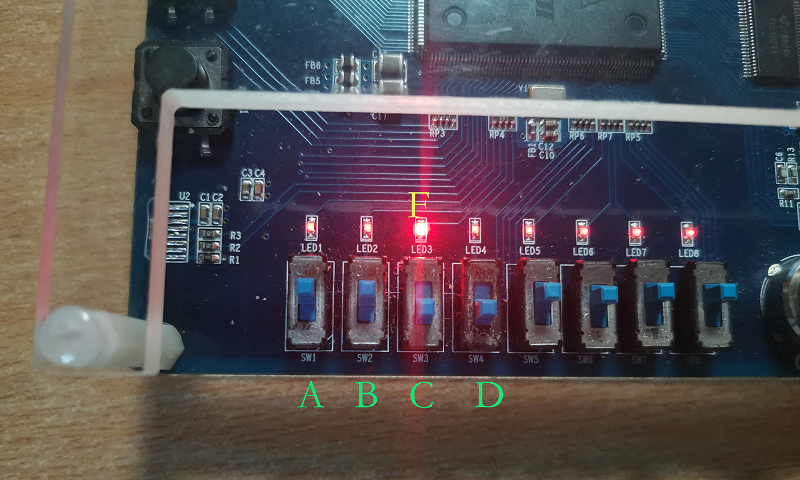
\includegraphics[scale=0.36]{3.png}}\hspace{0.3mm}
    \subfigure[4]{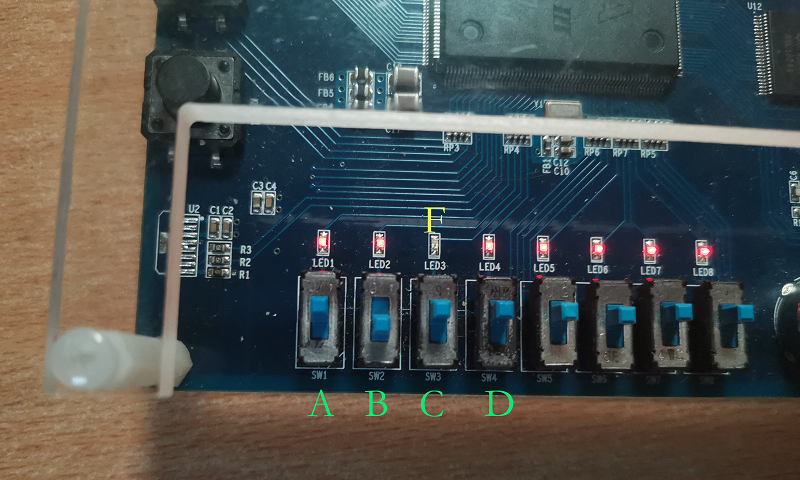
\includegraphics[scale=0.36]{4.png}}\hspace{0.3mm}
    \subfigure[5]{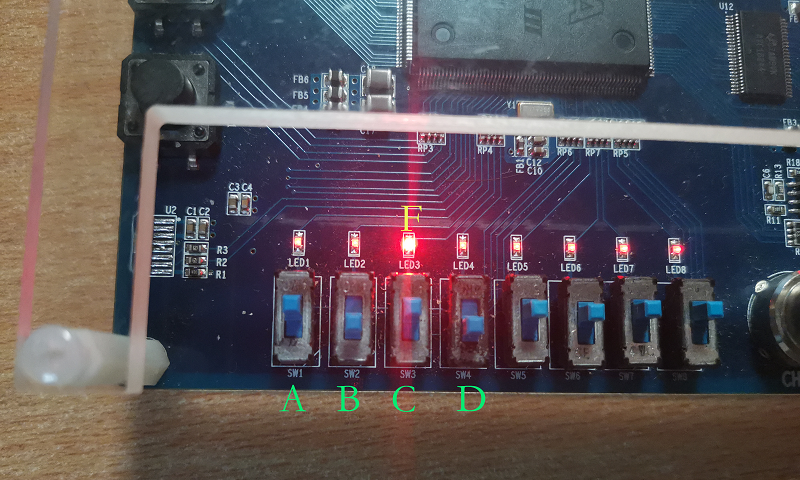
\includegraphics[scale=0.36]{5.png}}\hspace{0.3mm}
    \subfigure[6]{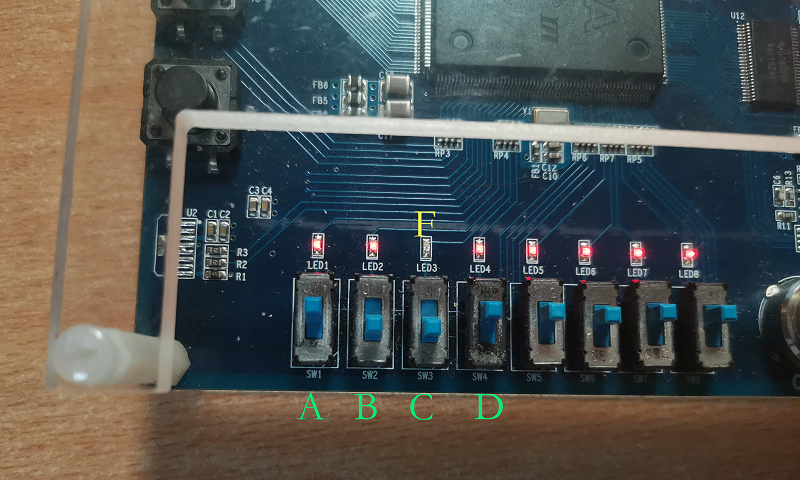
\includegraphics[scale=0.36]{6.png}}\hspace{0.3mm}
    \subfigure[7]{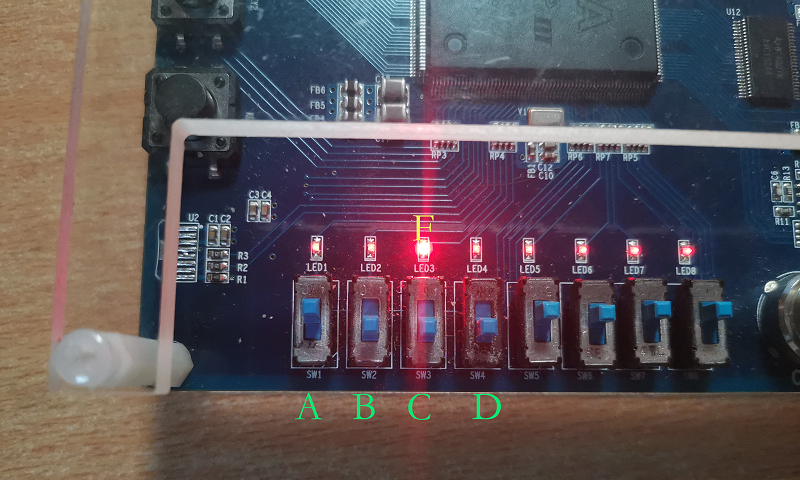
\includegraphics[scale=0.36]{7.png}}\hspace{0.3mm}
    \subfigure[8]{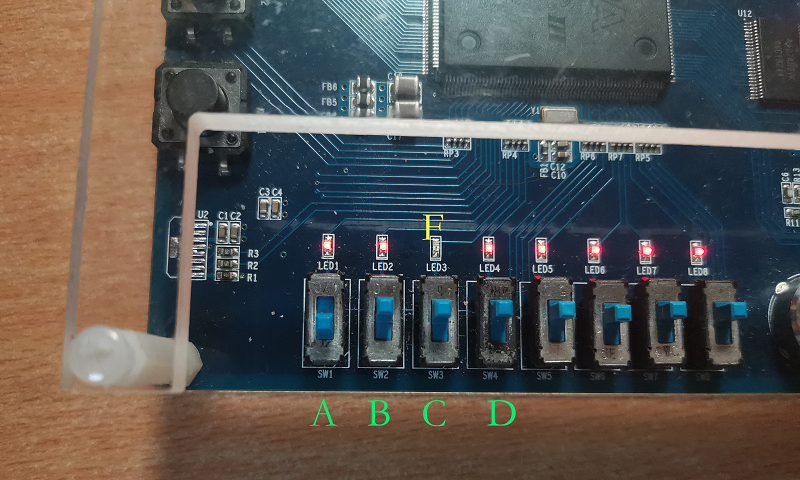
\includegraphics[scale=0.36]{8.png}}\hspace{0.3mm}
    \subfigure[9]{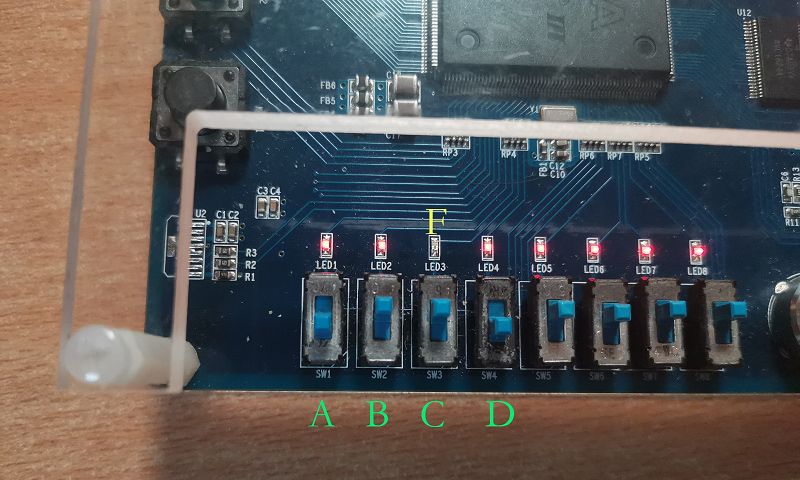
\includegraphics[scale=0.36]{9.png}}\hspace{0.3mm}
    \subfigure[10]{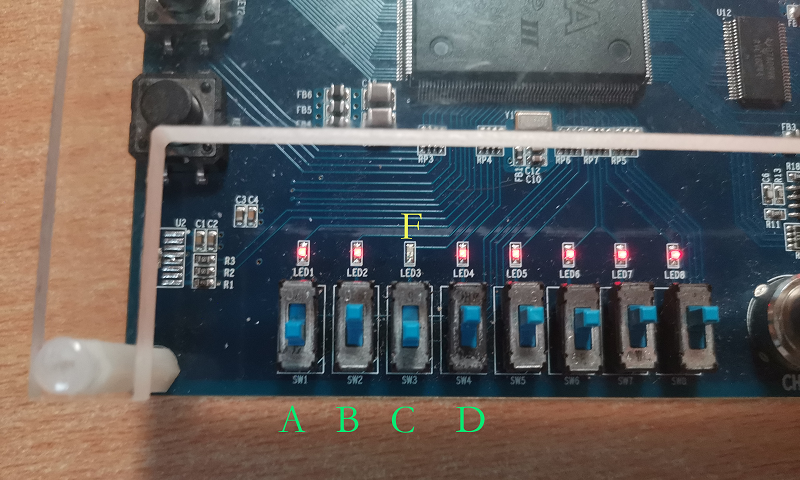
\includegraphics[scale=0.36]{10.png}}\hspace{0.3mm}
    \subfigure[11]{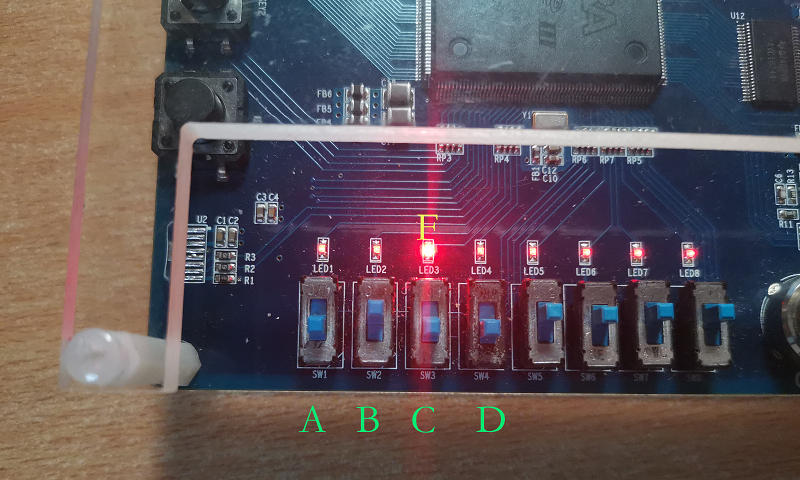
\includegraphics[scale=0.36]{11.png}}\hspace{0.3mm}
    \subfigure[12]{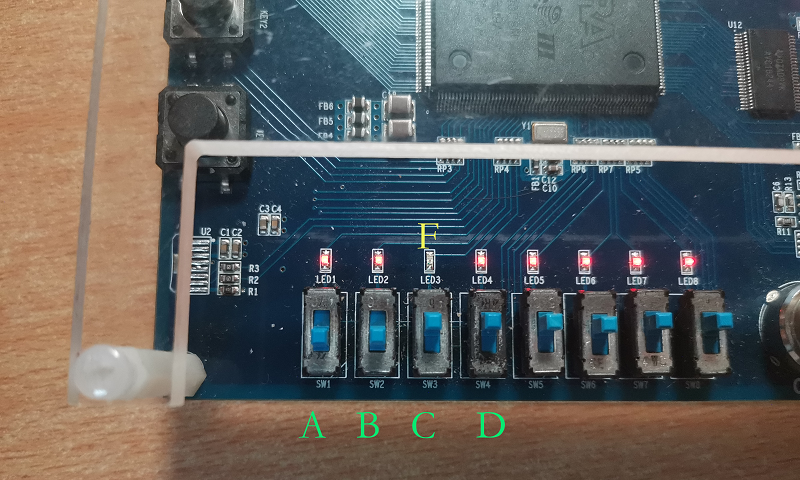
\includegraphics[scale=0.36]{12.png}}\hspace{0.3mm}
    \subfigure[13]{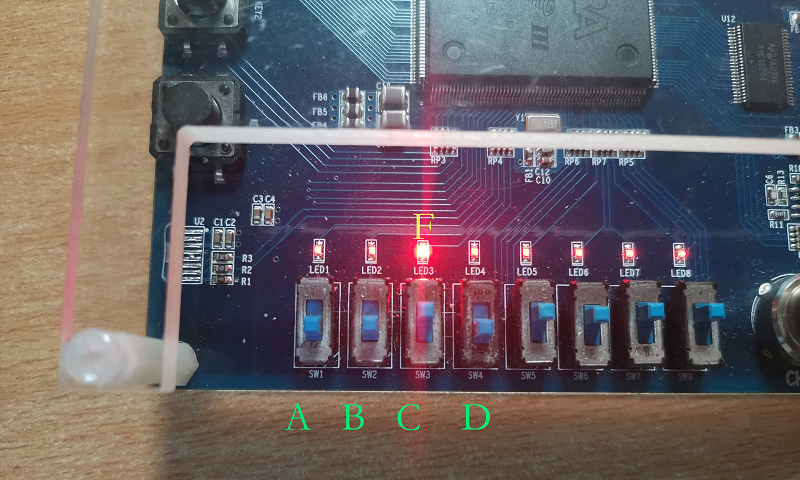
\includegraphics[scale=0.36]{13.png}}\hspace{0.3mm}
    \subfigure[14]{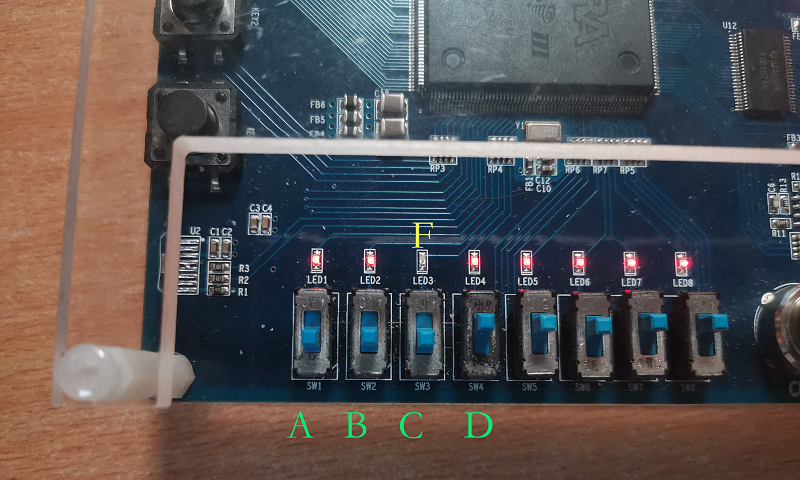
\includegraphics[scale=0.36]{14.png}}\hspace{0.3mm}
    \subfigure[15]{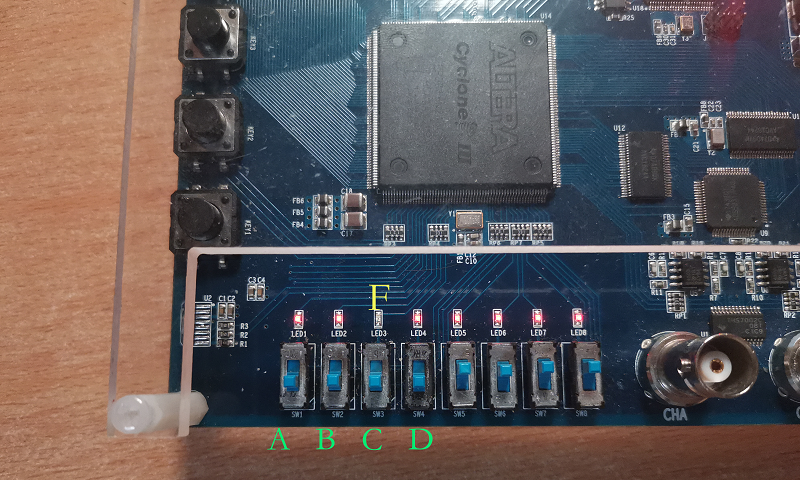
\includegraphics[scale=0.36]{15.png}}\hspace{0.3mm}
    \restoregeometry
    }
\end{figure}\par

\section{故障的解决及其他一些思考}
\subsection{线路图中线路未连接正确}
如果线路中断,则全编译时会给出错误提示
\begin{figure}[H]
    \centering{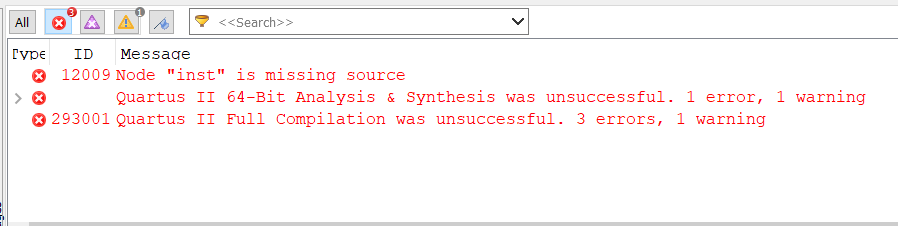
\includegraphics[scale=0.9]{error11.PNG}}
\end{figure}
"node'xx' is missing source"说明某节点并没有输入信号,仔细排查电路,发现电路图中部分线路有"x"标记,这说明电路中断,并未连接正确,如下图所示:
\begin{figure}[H]
    \centering{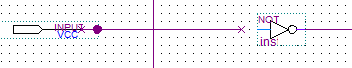
\includegraphics[scale=1.2]{error12.PNG}}
\end{figure}
此时只需要将未连接好的线路连接上即可。\par
另外,连接电路图中细线"node tool"和总线"bus tool"不可混用,否则也会显示电路中断的问题。

\subsection{仿真输入信号波形的技巧}
理想的输入信号应该是按照数字大小而从大到小输入"0000,0001,0010,...,1110,1111",这样可以更清晰地判断输入的数字数值,从而快捷地判断输出结果是否正确. 输入"A-D"信号时,需要注意A是二进制最高位,D是二进制最低位,因此我们将D的周期设为最短周期,先0后1;C周期为D的两倍,C取0和1时D分别变化一整周期;以此类推,从而得到理想输入信号波形。\par
除此之外,我们还可以将"A-D"信号设为一个group,并将进制设为"unsigned decimal",从而可以直观地看到输入的数字对应的十进制数。如下图所示:
\begin{figure}[H]
    \centering{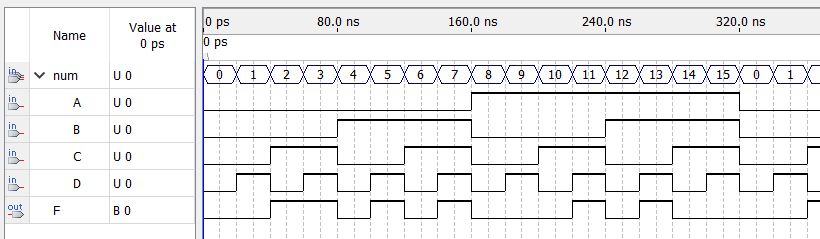
\includegraphics[scale=0.9]{wave.PNG}}
\end{figure}

\subsection{电路图另一种设计的讨论}
在实验过程中,我看到有部分同学改装电路时,看到原电路在判断$x=0-14$时结果均正确,只在$x=15$时出现错误,于是只需要特判$x=15$的情况,另$A=B=C=D=1$时$F$不能取1即可,将电路设计改造成了下图:
\begin{figure}[H]
    \centering{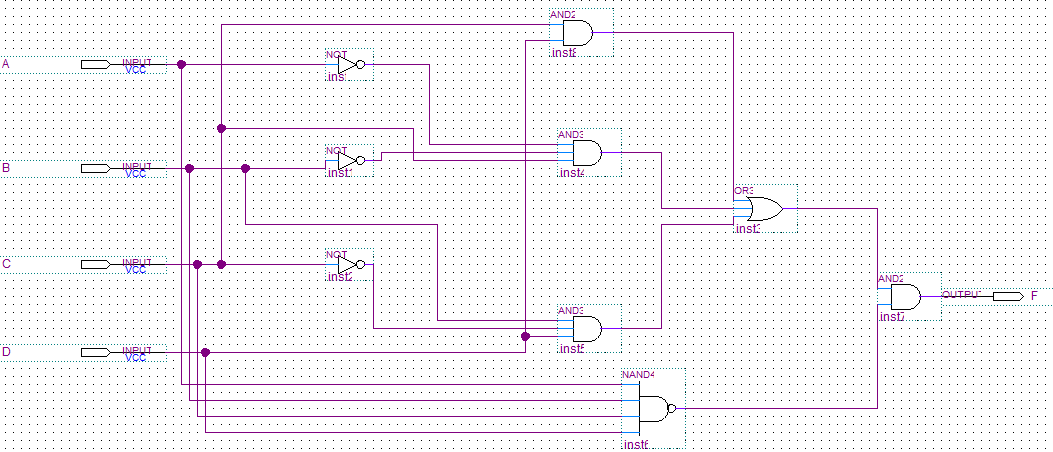
\includegraphics[scale=0.85]{curcuit2.PNG}}
\end{figure}
此种方法看似十分神奇,其实结合卡诺图我们就能清楚地明白原理:
\begin{table}[H]\begin{center}
    \begin{tabular}{|c|c c c c|}
        \hline
        \diagbox[width = 5em,height=2em]{AB}{CD}&00&01&11&10\\
        \hline
        00&0&0&1&1\\
        01&0&1&1&0\\
        11&0&1&0&0\\
        10&0&0&1&0\\
        \hline
    \end{tabular}
\end{center}\end{table}
原电路给出的做法是第2列2、3行合并得到BC'D,第3列整个合并得到CD,第1行3、4列合并得到A'B'C——可以明显看出"1111"项(第三行第三列)本来是0,这里也被当作了1进行卡诺图化简;于是我们只需再挖去这个点即可。因此细究这种电路图的连法,也能找到其理论依据。

\section{实验过程中的困难及其解决}
虽然理论课上详细学习了电路图、逻辑电路等相关知识,可到实际硬件应用时仍不免生疏,可见实践也是学习必要的一环。同时,我也感受到了理论的意义——最终,我们学习的知识都可以对应到实际的应用当中,这或许是知识最本质的意义。最后,在实践中出错、在实践中获得问题的其他思路(如用3.3用另一种电路图完成了实验要求),往往也会给理论的学习带来一定的启发——实践与理论相辅相成,不可分割。
\end{document}
